\documentclass[letterpaper,twocolumn,10pt]{article}
\usepackage{usenix2019_v3}
\usepackage{microtype}
\usepackage{booktabs}
\usepackage{tabularx}
\usepackage{graphicx}
\usepackage{xcolor}
\usepackage{amsmath}
\usepackage{xspace}
\usepackage{tikz}
\usetikzlibrary{arrows.meta,fit,positioning,shapes.geometric}
\newcommand{\system}{\textsc{ECPA}\xspace}
\newcommand{\code}[1]{\texttt{#1}}
\definecolor{ecpablue}{HTML}{DCEBFA}
\definecolor{ecpagreen}{HTML}{DFF1E3}
\definecolor{ecpaorange}{HTML}{FBE8CF}
\definecolor{ecpared}{HTML}{F7D8D8}
\definecolor{ecpagray}{HTML}{ECEFF3}
% Generated by paper/scripts/generate_evidence_summary.py; do not edit.
% Values are modeled/static or status evidence unless the paper says
% otherwise.
\newcommand{\ECPAWorkshopMods}{24}
\newcommand{\ECPAWorkshopBundleNamespace}{16}
\newcommand{\ECPAWorkshopTestPass}{17}
\newcommand{\ECPAWorkshopEnvironmentBlocked}{5}
\newcommand{\ECPAPlannerSeedExtensions}{11}
\newcommand{\ECPAAdaptationCandidates}{5}
\newcommand{\ECPAPlannerCases}{31}
\newcommand{\ECPAPlannerAdmits}{21}
\newcommand{\ECPAPlannerRejects}{10}
\newcommand{\ECPAPlannerRejectPrecision}{1.0}
\newcommand{\ECPAPlannerRejectRecall}{1.0}
\newcommand{\ECPAPlannerAdmitRecall}{1.0}
\newcommand{\ECPASourceRepositories}{15}
\newcommand{\ECPASourceObjects}{41}
\newcommand{\ECPAFormalCompleted}{1}
\newcommand{\ECPAFormalStarts}{9}
\newcommand{\ECPAFormalLifecycleSources}{5}
\newcommand{\ECPAHOneFalseEffectiveNumerator}{3}
\newcommand{\ECPAHOneFalseEffectiveDenominator}{3}
\newcommand{\ECPAHOneCoverage}{0.5}
\newcommand{\ECPAHTwoScoredCases}{5}
\newcommand{\ECPAHTwoTruePositive}{2}
\newcommand{\ECPAHTwoTrueNegative}{3}
\newcommand{\ECPAHTwoFalsePositive}{0}
\newcommand{\ECPAHTwoFalseNegative}{0}
\newcommand{\ECPAHTwoAdmitPrecision}{1.0}
\newcommand{\ECPAHTwoAdmitRecall}{1.0}
\newcommand{\ECPAHTwoRejectPrecision}{1.0}
\newcommand{\ECPAHTwoRejectRecall}{1.0}
\newcommand{\ECPAHTwoAcceptedOrders}{2}
\newcommand{\ECPAHTwoCompressionOrders}{2}
\newcommand{\ECPAHTwoCompressionSemanticTokens}{1201}
\newcommand{\ECPAHTwoCompressionPhysicalTokens}{1024}
\newcommand{\ECPAHTwoCompressionWorkerAcks}{2}
\newcommand{\ECPAFormalPlanned}{30}
\newcommand{\ECPAVerifiedAdapters}{3}
\newcommand{\ECPAReferenceStarts}{45}
\newcommand{\ECPAFormalArms}{3}
\newcommand{\ECPAMinimumStarts}{3}
\newcommand{\ECPAScheduleRows}{3}
\newcommand{\ECPAResearchClaims}{4}
\newcommand{\ECPAFirstStudyStarts}{9}
\newcommand{\ECPADeploymentBlockers}{0}
\newcommand{\ECPARegisteredDeploymentArms}{3}
\newcommand{\ECPATransactionModelStates}{39}
\newcommand{\ECPATransactionModelEdges}{102}
\newcommand{\ECPATransactionModelRejections}{522}
\newcommand{\ECPATransactionModelInvariants}{7}
\newcommand{\ECPAReleaseVersion}{0.3.0}
\newcommand{\ECPAManifestVersion}{0.3}
\newcommand{\ECPAReleaseDistributions}{36}
\newcommand{\ECPAReleaseRegistrations}{39}
\newcommand{\ECPAReleaseActivationIntent}{24}
\newcommand{\ECPAReleaseInspectOnly}{15}
\newcommand{\ECPAReleaseGates}{9}
\newcommand{\ECPANativeLifecycleQualifications}{1}

% Generated from the complete real R4 archive; finite nonformal evidence.
\newcommand{\ECPAAttentionSourceRecords}{261}
\newcommand{\ECPAAttentionWorkerClosures}{2}
\newcommand{\ECPAAttentionCompletionReceipts}{56}

\raggedbottom
\setlength{\emergencystretch}{2em}
\def\UrlBreaks{\do\/\do-\do\_}
\sloppy
\hbadness=10000
\title{\Large \bf From Enabled to Effective: Evidence-Bound Activation for LLM Inference Extensions}
\author{Anonymous Submission}
\date{}

% Internal accountability (excluded from the anonymized author line):
% ShuhaoZhangTony / 张书豪 is the PI lead and accountable executor. Student
% participation is optional and non-blocking.

\begin{document}
\pagestyle{plain}
\maketitle

\begin{abstract}
Modern LLM inference engines continually add KV-cache management, preemption,
offload, tiered storage, scheduling, observability, and disaggregated serving.
These extensions increasingly enter through forks, hard-coded hooks, or
package entry points, which establish discovery and loading but do not show
that independently developed extensions compose correctly or affect every
process that can serve a request. This gap creates \emph{false-effective}
states: deployment state reports success while workers execute a partial,
stale, inert, or conflicting configuration. We present ECPA, an inference-system
extension contract and runtime. Contracts declare capabilities, resource and
lifecycle authority, dependencies, process coverage, failure policy, and
verifiable effect conditions. A compiler turns multiple contracts into an
immutable execution plan; the protocol orders prepare, activate, observe,
expose, and rollback phases. Authority-owned evidence discharges
plan obligations, and the design specifies an ExposureGate that should make a
generation externally visible only after fresh evidence covers its
epoch-scoped targets.  A separate real TP2 qualification demonstrates
invocation-coverage admission and revocation through an independent HTTP
authority; formal traffic-boundary prevention remains unestablished.  We derive the model
from the plugin page's source-bound population of \ECPAWorkshopMods{} MODs,
spanning scheduling, speculative decoding, KV data paths, model execution,
communication, and observability.  We implement a host-neutral
coordinator, a narrow adapter for one vLLM-compatible prototype host, and an
adversarial evaluation harness covering namespace errors, resource conflicts,
partial worker coverage, replay, crash recovery, lease expiration, and failed
compensation.  The first preregistered real-host study ran nine independent
cold TP2 starts across entry-point, manual-integration, and ECPA arms.  All
nine records passed offline evidence validation, but after one worker's
evidence was quarantined, all three ECPA repetitions still claimed effective
with only 0.5 process coverage.  This falsifies the tested H1 prevention claim
and identifies independent traffic-boundary enforcement as a system requirement.
The later invocation-only qualification does not change this falsification.  The study makes no
throughput, latency, rollback, or cross-runtime claim.  A separate
source-bound H2 subset currently scores \ECPAHTwoScoredCases{} definite
compositions ($TP=\ECPAHTwoTruePositive{},TN=\ECPAHTwoTrueNegative{},
FP=\ECPAHTwoFalsePositive{},FN=\ECPAHTwoFalseNegative{}$).  Its observed
precision and recall are 1.0, but this
sample is too small and omits important conflict surfaces, so H2 remains open.
\end{abstract}

\section{Introduction}
Plugins are becoming the de facto change boundary for fast-moving inference
systems.  A scheduler policy may be delivered as a Python entry point; a KV
connector may depend on an external service; a production-stack adapter may
translate intent into Kubernetes configuration; and a provider may map a
portable capability to a host-specific command-line flag.  This modularity is
valuable, but it creates a gap between packaging facts and runtime facts.

Consider an operator who installs a plugin distribution, sees its configuration
saved, enables it, and launches an engine with multiple worker processes.  The
parent process may discover the distribution while one worker imports a
different version, never invokes the hook, or lacks the provider.  Two plugins
may independently validate yet both claim the same KV connector option.  An
external service may fail after intent is persisted.  Conventional loaders
often collapse these cases into an ``enabled'' bit.  That bit is useful intent,
but it is not evidence that the plugin changed the running system.

The repository that motivated this work contains a smaller but revealing
incident.  A one-line ``bugfix'' changed discovery from the host-owned static
bundle namespace to an upstream-looking namespace.  Sixty-six unit tests still
passed.  Yet an installed KV-connector provider registered one bundle in the
declared namespace, the modified manager selected zero entries, and discovery
returned no bundles.
Installation succeeded; the code imported; runtime intent could still exist;
the plugin was nevertheless absent from the activation path.  The incident is
not important because of the spelling error itself.  It demonstrates that
tests and static state can agree while authority and runtime effect disagree.

We ask: \emph{how can an inference system make extensions discoverable,
composable, verifiable, and rollback-safe when runtime effectiveness cannot be
proved statically?}  We build \system, an extension contract and transactional
runtime centered on evidence-bound activation.  The Extension Manager is its
reference implementation; the contract, corpus, and conformance suite define
what another implementation must reproduce.  A decision is not ``enable plugin $p$'' but an activation plan
for a concrete host version, provider set, plugin set, process topology, and
resource-ownership graph.  The plan records evidence obligations.  Each
obligation must be discharged by its declared authority; a plan-bound process
invocation can discharge only its corresponding process or invocation
obligation.  A manager cannot manufacture runtime effectiveness from
configuration.

Figure~\ref{fig:architecture} summarizes this split: portable contracts and
transactions stop at a typed adapter, while host and provider authorities send
effect evidence back across that boundary.  Neither the adapter nor an
individual plugin can open the traffic gate by self-report.

Our intended safety property is: \emph{no activation is exposed as effective unless
every required plan obligation in the current epoch has fresh evidence from
the authority that can observe its planned effect}.  Process-scoped obligations
also require coverage of their frozen target set.  ECPA is not the first
plugin system, a deployment controller, or a software-supply-chain attestation
scheme.  Its contribution is an evidence-bound activation protocol for
extensions whose effect spans multiple inference processes and authority
domains.  Existing plugin APIs, controllers, and provenance systems are inputs
to that protocol, not components that ECPA replaces.  The completed H1 cell
shows that the reference runtime does not yet realize this property, so the
present contribution is the contract, protocol, and falsifiable test method,
not a validated prevention mechanism.

The contract, compiler, coordinator, and evidence protocol do not name a host
runtime or plugin package.  We evaluate them through a deep study on one
vLLM-compatible prototype host, connected only through a typed host adapter.
Within that host we cover multiple independently implemented extension classes,
parent/engine/worker process scopes, versions and topologies, authority
boundaries, and fault modes.  This is single-host evidence, not a claim of
cross-framework validation; a second runtime is future external-validity work.

This paper makes three contributions, with claim strength bounded by
the evidence available today:
\begin{itemize}
  \item an inference-extension contract that expresses capabilities,
  resources, lifecycle authority, dependencies, process coverage, and
  machine-checkable effect obligations rather than only loadable APIs;
  \item a contract compiler and transactional runtime that produce immutable
  execution plans and define multi-process prepare, activation, exposure,
  replacement, failure, and rollback semantics; and
  \item a host-evidence model and independent evaluation method for detecting
  false-effective extensions across correctness, conflict, skew, recovery,
  multi-process consistency, and overhead experiments.
\end{itemize}
The contract compiler, reference coordinator, evidence protocol, and
fail-closed formal harness are implemented.  Release \ECPAReleaseVersion{}
freezes Manifest \ECPAManifestVersion{} and records one pinned native-host
lifecycle qualification.  The source-bound static corpus is measured, and the
first matched prototype-host H1 cell is complete and falsifies its prevention
hypothesis.  H2 has a \ECPAHTwoScoredCases{}-case real-source subset but lacks the breadth to
support its population claim; H3 and H4 each have zero formal runs.  A real
authority-owned HTTP route now has invocation-only qualification, while its
formal prevention and effect-semantics evaluation remains incomplete.  We do not present
modeled decisions, interface fixtures, release qualification, or lifecycle
startup fields as substitutes for those experiments.

\begin{figure*}[t]
\centering
\resizebox{\textwidth}{!}{%
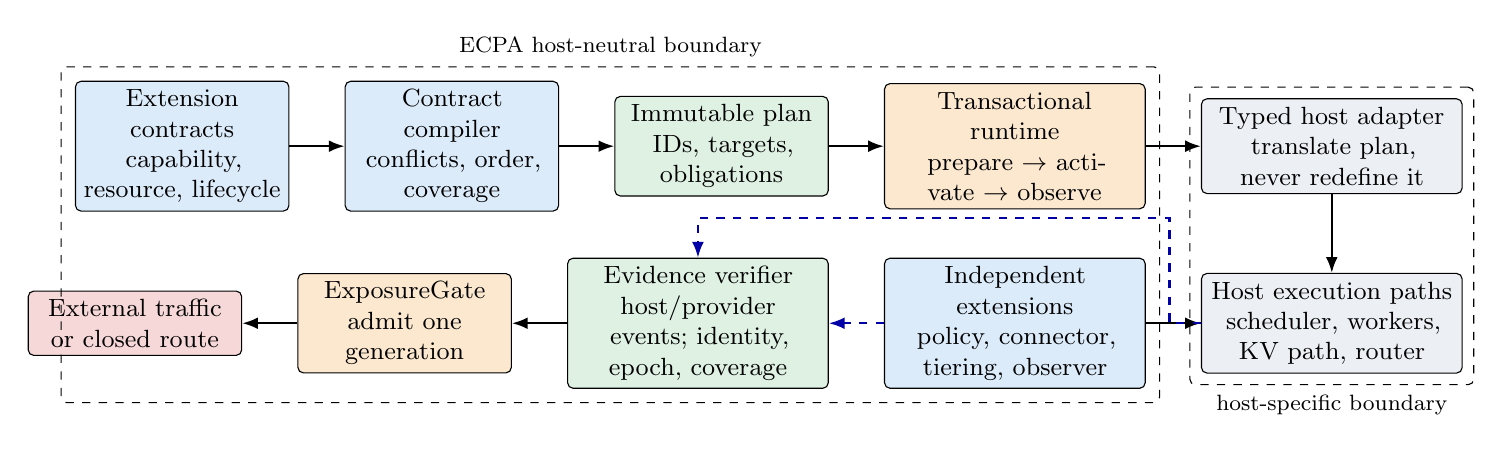
\begin{tikzpicture}[
  font=\small,
  node distance=5mm and 7mm,
  box/.style={draw, rounded corners=2pt, align=center, minimum height=8mm,
    text width=25mm, inner sep=3pt},
  wide/.style={box, text width=31mm},
  flow/.style={-{Latex[length=2mm]}, thick},
  evidence/.style={-{Latex[length=2mm]}, thick, dashed, color=blue!65!black}
]
\node[box, fill=ecpablue] (contracts) {Extension contracts\\capability, resource, lifecycle};
\node[box, fill=ecpablue, right=of contracts] (compiler) {Contract compiler\\conflicts, order, coverage};
\node[box, fill=ecpagreen, right=of compiler] (plan) {Immutable plan\\IDs, targets, obligations};
\node[wide, fill=ecpaorange, right=of plan] (runtime) {Transactional runtime\\prepare $\rightarrow$ activate $\rightarrow$ observe};
\node[wide, fill=ecpagray, right=of runtime] (adapter) {Typed host adapter\\translate plan, never redefine it};

\node[wide, fill=ecpagray, below=10mm of adapter] (paths) {Host execution paths\\scheduler, workers, KV path, router};
\node[wide, fill=ecpablue, left=of paths] (extensions) {Independent extensions\\policy, connector, tiering, observer};
\node[wide, fill=ecpagreen, left=of extensions] (verify) {Evidence verifier\\host/provider events; identity, epoch, coverage};
\node[box, fill=ecpaorange, left=of verify] (gate) {ExposureGate\\admit one generation};
\node[box, fill=ecpared, left=of gate] (traffic) {External traffic\\or closed route};

\draw[flow] (contracts) -- (compiler);
\draw[flow] (compiler) -- (plan);
\draw[flow] (plan) -- (runtime);
\draw[flow] (runtime) -- (adapter);
\draw[flow] (adapter) -- (paths);
\draw[flow] (extensions) -- (paths);
\draw[evidence] (paths.west) -- ++(-4mm,0) |- ([yshift=5mm]extensions.north) -| (verify.north);
\draw[evidence] (extensions.west) -- (verify.east);
\draw[flow] (verify) -- (gate);
\draw[flow] (gate) -- (traffic);

\node[draw, dashed, rounded corners=2pt, fit=(adapter)(paths), inner sep=4pt,
  label={[font=\footnotesize]below:host-specific boundary}] {};
\node[draw, dashed, rounded corners=2pt, fit=(contracts)(compiler)(plan)(runtime)(verify)(gate),
  inner sep=5pt, label={[font=\footnotesize]above:ECPA host-neutral boundary}] {};
\end{tikzpicture}
}
\caption{ECPA separates portable extension semantics from a narrow host adapter.
The adapter maps an immutable plan into native execution paths; it cannot
declare success.  Effect evidence returns from the authority that can observe
each obligation, and only the ExposureGate can make a generation visible.}
\label{fig:architecture}
\end{figure*}

\section{Background and Motivation}
\subsection{Why Existing State Is Ambiguous}
A package manager proves that files exist.  Entry-point discovery proves that
metadata contains a name.  Configuration proves that an operator supplied
parameters.  An enabled bit proves desired intent.  None proves that the
selected implementation executed in every process that matters.  Conversely,
an external service can become unreachable while enabled intent should remain
for diagnosis and later recovery.  A linear state machine both overclaims
success and destroys useful failure context.

Vanilla entry points provide a deliberately lightweight extension mechanism
\cite{vllm-plugin}.  Manual integration can add flags, environment variables,
and operator checks.  Both are legitimate baselines.  Their limitation is not
that they can never be made safe; it is that evidence obligations, ownership,
and rollback are convention rather than a common machine-checkable contract.

\section{Problem and Formal Model}
\subsection{System Model}
We model a host runtime $H$, providers $P$, plugins $G$, processes $W$, and
resources $R$.  A plugin manifest declares required and provided capabilities,
version predicates, claimed resources, provider needs, and evidence
obligations.  A provider translates an accepted plan into host-specific
configuration, but it does not supervise the host or acquire authority over an
external service.  Each launch has a unique identity $\ell$ and an expected
process set $W_\ell$.

An activation plan $A=(H,P,G,W,R,V)$ is admissible only if capability
requirements resolve under a frozen public-PEP-440 comparison profile,
resource ownership is conflict-free or mediated by a selected claimant, and
every evidence obligation names an exact role/event/direction/capability
authority grant and its selected capability provider plus, when applicable, a
positive quorum threshold.  Let $O_A^{required}$ be the required process,
resource, provider-operation, and external-authority obligations compiled into
$A$, and let $E$ be the observed evidence set.  Runtime effectiveness is:
\begin{equation*}
effective(A,\ell,E) \iff
\forall o \in O_A^{required}: complete(o,A,\ell,E).
\end{equation*}
Each completion predicate checks the obligation's authority, identity,
freshness, and value; process obligations additionally check membership or an
explicit positive quorum.  The manager may not silently remove an obligation
or weaken its predicate.

ECPA deliberately separates five facts that conventional extension state often
collapses.  $D(p)$ means a contract declares extension $p$; $P(p,A)$ means an
admissible immutable plan selects it; $I(p,w,A,\ell)$ means a plan-bound host
path invoked it in process $w$; $F(A,\ell,E)$ abbreviates the effectiveness
predicate above; and $X(A,\ell)$ means the ExposureGate admitted the generation
to external traffic.  Compilation ensures $P\Rightarrow D$, valid invocation
evidence ensures $I\Rightarrow P$, and the gate enforces $X\Rightarrow F$.
No reverse implication is assumed, and $F$ does not reduce to $I$: a plan can
also require resource effects, provider operations, and external-authority
facts.  Loading is therefore an activation event, not an effectiveness
verdict.  A false-effective outcome is
\begin{equation*}
reported\_effective(A,\ell) \land \neg F(A,\ell,E),
\end{equation*}
where the right-hand side is computed from the preregistered target and
obligation sets together with authority-owned observations, rather than from
the manager's status bit.

\begin{table}[t]
\centering\small
\caption{Extension facts and the authority permitted to establish them.}
\begin{tabularx}{\columnwidth}{@{}lXX@{}}
\toprule
Fact & Evidence & Owning authority \\
\midrule
Declared & static manifest and distribution metadata & package registry \\
Planned & immutable plan and resolved provider graph & contract compiler \\
Invoked & launch-bound hook or dispatch event & host execution path \\
Effective & every required obligation completes & obligation authorities \\
Exposed & generation admitted to external traffic & ExposureGate \\
\bottomrule
\end{tabularx}
\end{table}

\subsection{Threat Model}
We address accidental incompatibility, stale or replayed evidence, conflicting
ownership, provider ambiguity, parent/worker version mismatch, partial rollout,
observer loss, process crashes, and interrupted rollback.  Plugins and
providers may be buggy and may report inconsistent metadata.  We assume the
host, package database, and process identity channel are administratively
trusted.  We do \emph{not} sandbox malicious Python, defend a compromised host,
or claim that signed metadata makes arbitrary plugin code safe.  This boundary
follows the upstream warning that plugins execute with application authority
\cite{vllm-security}.
The formal harness trusts the experiment host, runner, registered lifecycle
sources, and registry-pinned observer, but not SUT acknowledgements or
telemetry. It does not defend against malicious same-user code inspecting
descriptors or rewriting artifacts. Five distinct sources own readiness,
workload, fault, host-effect, and shutdown facts. Their challenge-bound receipts
carry plan/launch/invocation and PID/start-time identities over
kernel-credentialed Unix channels; an ACK alone proves none of these facts.
Formal observables carrying \code{causal\_ack} are rejected.
The host observer reads a host-owned journal and cannot stand in for the other
sources. Fixture services and their artifacts cannot enter the formal
aggregate. These checks make records runner-consistent within the stated trust
boundary, not cryptographic attestations against a malicious SUT.

\subsection{Invariants and Failure Semantics}
\system enforces four invariants.  \textbf{I1, evidence monotonicity:} a stronger
state requires new evidence and cannot be inferred from a weaker state.
\textbf{I2, single explicit ownership:} every exclusive resource has one owner
or a declared mediator.  \textbf{I3, authority locality:} evidence is accepted
only from the component that can observe the claimed event.  \textbf{I4,
rollback preservation:} no new plan destroys the last committed valid plan
before the replacement satisfies its commit gate.

Failures are structured outcomes, not booleans.  A missing provider or
unsupported version makes a plan inadmissible.  A service outage can preserve
\emph{enabled} intent while marking health degraded and refusing a new launch.
A missing worker attestation leaves the activation partial, never globally
effective.  Stale evidence is rejected by launch, process, host, manifest, and
runtime-version identity.  Rollback either restores the recorded predecessor
or reports a bounded operator action; it never invents success.

\subsection{Safety Argument}
Assume that plan publication and generation compare-and-swap are atomic, each
evidence source belongs to its declared administrative authority, the channel
preserves sender identity, and target membership is frozen for one process
epoch.  Then an ECPA-controlled route
cannot expose a candidate generation before all of its required obligations
are satisfied.  The planner fixes the obligations and target set in the plan
digest.  Evidence validation rejects a different plan, launch, controller,
process epoch, target identity, or invocation sequence.  The ExposureGate
opens only for that digest after the validator reports a complete set, and its
route fence names the same generation.  A delayed validator or controller
therefore fails the generation compare-and-swap rather than opening a newer
route.

This conditional argument concerns admission, not functional correctness.
A source closure inside an acknowledged prefix bounds a finite observation;
it does not keep an effect valid after process replacement or evidence expiry.
Continuing admission requires epoch fencing and an explicit invalidation policy.
False semantic events from authorized sources or undeclared effects invalidate
the premises.  Rollback closes the candidate before restoring its predecessor;
it cannot restore external state the manager does not own.  These boundaries
require independent observers and fault injection.

We also encode the declared exposure transaction as a finite abstract model.
Exhaustive fixed-point exploration reaches \ECPATransactionModelStates{} states
and \ECPATransactionModelEdges{} valid edges, while rejecting
\ECPATransactionModelRejections{} invalid state-action pairs.  None of the
reachable states violates its \ECPATransactionModelInvariants{} checked
invariants, including no candidate admission before a proof-bound open receipt,
no admission in failed-safe or safety-unknown states, and predecessor-only
strong rollback.  This is evidence about the stated abstraction under its
recorded assumptions, not a proof that the implementation refines the model or
that a real prototype-host deployment recovers correctly.  H3 therefore remains a
planned formal-real claim.

\subsection{Refinement Boundary}
The safety claim spans three representations that must not be conflated.  The
contract compiler produces a canonical plan and obligation set; the durable
coordinator records an intended state transition; and the traffic authority
controls the externally observed route.  Let durable coordinator state be
$S=(g,q,p,c,f,\pi)$, where $g$ is the candidate generation, $q$ the lifecycle
state, $p$ and $c$ the predecessor and candidate digests, $f$ the route fence,
and $\pi$ the accepted proof digest.  Let the traffic authority report
$R=(g_r,f_r,d_r)$ for its observed generation, fence, and route snapshot
digest.  The abstract predicate \emph{exposed} is represented only when
\begin{equation*}
\begin{aligned}
q &= \textsc{CandidateOpen}, \\
(g_r,f_r,d_r) &= (g,f,c), \qquad valid(\pi,g,c).
\end{aligned}
\end{equation*}
A database row alone is therefore not an exposure fact, and a route mutation
alone is not a committed transition.

The reference implementation uses an intent--effect--query--receipt protocol
at every authority-crossing transition.  It first commits a transition intent,
invokes the traffic adapter, queries the adapter's actual route, and commits a
receipt only if generation, fence, and snapshot digest match.  Recovery treats
an intent without a receipt as an uncertain operation and reconciles it from a
fresh route query.  A failed or unobservable close enters \textsc{SafetyUnknown}
rather than manufacturing fail-closed success.  Table~\ref{tab:refinement}
states the refinement obligations explicitly; passing the finite abstract
model establishes none of them by itself.

\begin{table}[t]
\centering\small
\caption{Refinement obligations between the abstract transaction and the
reference implementation.}
\label{tab:refinement}
\begin{tabularx}{\columnwidth}{@{}lX@{}}
\toprule
Obligation & Implementation boundary and falsification test \\
\midrule
R1: plan immutability & Bind the canonical plan and target digest before
activation.  Falsify with mutation and mixed-generation inputs. \\
R2: evidence binding & Insert a receipt only after identity, authority, epoch,
and coverage checks.  Falsify with replay, source substitution, and PID reuse. \\
R3: exposure agreement & Query the traffic authority and match the proof-bound
generation, fence, and snapshot before an open receipt.  Crash at each
intent/effect/query boundary. \\
R4: stale-writer exclusion & Bind a lease token and durable revision
compare-and-swap.  Recreate the manager, expire the lease, and delay a writer. \\
R5: recovery conservatism & Reconcile unmatched intents from the traffic
authority and block unknown routes.  Lose the query and fail compensation. \\
\bottomrule
\end{tabularx}
\end{table}

These obligations separate the theorem we want from the implementation we
have.  R1--R5 are exercised today only by the single-host reference gate and
its fault-injection suite.  Establishing them for the prototype host requires the
registered formal-real adapter, host-owned process evidence, and a real traffic
authority.  Until then, the artifact supports an abstract safety result and a
reference-implementation conformance result, not an end-to-end refinement
claim.

\section{Design}
\subsection{Typed Static Manifests}
Discovery reads distribution metadata and a static manifest without importing
implementation modules.  The schema distinguishes bundle identity, component
kind, semantic capability, host/API range, provider, required service, resource
claims, and activation/evidence contracts.  Static discovery avoids executing
plugin code merely to decide whether it is eligible.  Namespace ownership is
typed and parameterized by the host profile: a manifest names the owning
authority and exact registration group; an adapter may delegate to a
host-native hook but may not mint a group owned by another authority.  No
namespace or package prefix is built into the ECPA schema.

The namespace incident becomes a schema fixture: package metadata must contain
exactly the declared group and bundle identity, and a clean installed-package
probe must observe it.  This closes the test gap that allowed a constant to
change while mock-based tests continued to pass.

\subsection{Capability Negotiation}
Capabilities name semantics rather than package names.  A plugin can require a
versioned preemption-policy interface, a connector contract, or process-owned
invocation evidence.  The host and providers advertise concrete capabilities
with provenance.  Negotiation produces a graph whose edges explain which
authority satisfies each requirement.  Missing, ambiguous, or incompatible
edges reject activation.  Untested version tuples remain \emph{unverified}, not
implicitly compatible.

\subsection{Conflict Planning}
Plugins claim resources such as a command-line/configuration key, hook slot,
scheduler policy, connector, service endpoint, or deployment field.  The
planner constructs an ownership graph and detects duplicate exclusive claims,
incompatible values, and conditional conflicts.  For example, two plugins that
both write \code{--kv-transfer-config} conflict even if their package names and
providers differ.  Two plugins sharing a read-only health provider need not
conflict.  The output is a deterministic, reviewable plan rather than an
order-dependent sequence of mutations.

\subsection{Contract Compilation and Plan Identity}
The compiler normalizes version predicates and identifiers, resolves each
requirement to one selected provider, topologically orders dependencies, and
checks resource claims against typed ownership modes.  It then expands
lifecycle declarations into process-specific evidence obligations.  The
canonical serialization freezes plugin versions, provider choices, host
compatibility, configuration digests, target roles, ordering, and failure
policy under one plan ID.  Every launch adds a fresh launch ID and process
epoch without changing the compiled semantics.

This compilation boundary provides a limited static guarantee: an admitted
plan has no unresolved requirement, dependency cycle, ghost mediator, or
multiply owned exclusive resource under the declared taxonomy.  It cannot show
that a hook executes, that a provider mutates the intended resource, or that
the taxonomy captures every semantic interaction.  Those are explicit runtime
or evaluation obligations rather than hidden assumptions of the compiler.

\subsection{Explicit Lifecycle}
Operator intent is not evidence state.  Its durable vector is:
\begin{center}
\code{installed, configured, enabled}.
\end{center}
Installed is distribution evidence; configured is validated saved input;
enabled is durable operator intent.  The separate evidence predicates are
declared, planned, invoked, effective, and exposed.  In particular,
runtime-effective means that every required plan obligation is complete, not
merely that an implementation ran.  Reachability, health, degradation, and
compatibility are orthogonal projections.  Thus an external outage does not
erase intent, and saved intent does not certify a running process.

\subsection{Authority- and Host-Owned Runtime Evidence}
Each activation plan emits obligations keyed by launch identity, authority,
process role or resource, plugin/component digest, host/runtime version, and
capability.  A worker (or an observer in its authority domain) records load and
invocation events; provider and external obligations name their own completion
sources.  The aggregator verifies identity, freshness, authority, expected
membership, and every declared completion predicate.  Parent-process import is
insufficient for a worker-side hook, and invocation alone is insufficient for a
declared resource or provider effect.  Evidence is compact lifecycle telemetry,
not prompt content.

In the running example, the static probe rejects the wrong namespace before
launch.  If static discovery succeeds but one worker never invokes the hook,
the plan may remain enabled and partially loaded, but cannot become globally
runtime-effective.  This same distinction covers inert imports and mixed
worker versions without special-case status strings.

\subsection{Fail-Closed Activation and Deterministic Rollback}
Planning is side-effect free.  Activation proceeds through prepare, validate,
activate, observe, expose, and commit; shutdown and rollback are explicit
terminal or compensating paths (Figure~\ref{fig:transaction}).  Exposure is distinct from activation: a
candidate may run behind a closed gate while obligations accumulate, but it
cannot receive external traffic until the gate accepts its complete identity
and evidence set.  Missing required services, contradictory capabilities, or
incomplete evidence stop before exposure.  The manager stores the canonical
predecessor plan, rendered inputs, version identities, and authority owners.
Rollback re-renders that predecessor and requires its own evidence gate.
External-service lifecycle remains operator-owned; rollback can restore client
configuration without pretending to downgrade a service it does not control.

\begin{figure}[t]
\centering
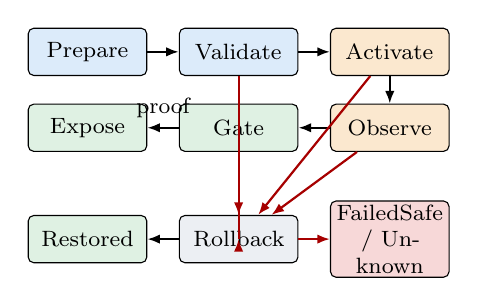
\begin{tikzpicture}[
  font=\footnotesize,
  node distance=3.5mm and 4mm,
  state/.style={draw, rounded corners=2pt, align=center, minimum height=6mm,
    text width=14mm, inner sep=1.5pt},
  flow/.style={-{Latex[length=1.6mm]}, thick},
  fail/.style={-{Latex[length=1.6mm]}, thick, color=red!65!black}
]
\node[state, fill=ecpablue] (prepare) {Prepare};
\node[state, fill=ecpablue, right=of prepare] (validate) {Validate};
\node[state, fill=ecpaorange, right=of validate] (activate) {Activate};
\node[state, fill=ecpaorange, below=of activate] (observe) {Observe};
\node[state, fill=ecpagreen, left=of observe] (gate) {Gate};
\node[state, fill=ecpagreen, left=of gate] (expose) {Expose};
\node[state, fill=ecpagray, below=8mm of gate] (rollback) {Rollback};
\node[state, fill=ecpagreen, left=of rollback] (restored) {Restored};
\node[state, fill=ecpared, right=of rollback] (unknown) {FailedSafe / Unknown};

\draw[flow] (prepare) -- (validate);
\draw[flow] (validate) -- (activate);
\draw[flow] (activate) -- (observe);
\draw[flow] (observe) -- (gate);
\draw[flow] (gate) -- node[above]{proof} (expose);
\draw[fail] (validate) |- (rollback);
\draw[fail] (activate) -- (rollback);
\draw[fail] (observe) -- (rollback);
\draw[fail] (gate) -- (rollback);
\draw[flow] (rollback) -- (restored);
\draw[fail] (rollback) -- (unknown);
\end{tikzpicture}
\caption{Activation is a transaction, not a callback list.  External traffic
remains closed through observation and proof validation.  Any pre-exposure
failure enters explicit compensation; unverifiable compensation is reported as
safety-unknown rather than success.}
\label{fig:transaction}
\end{figure}

\subsection{Authority Separation}
Core owns manifests, intent, planning, and evidence validation.  Providers own
translation and provider-specific checks.  The runtime owns process execution
and invocation facts.  External operators own services, clusters, drivers, and
data.  A provider protocol exposing plan/render/check therefore cannot silently
apply, delete, or restart infrastructure.  This separation limits both failure
blast radius and the claims that status may make.

\section{Durable Coordinator}
The reference coordinator is written in Python, but \system is not synonymous
with its package or prototype host.  It comprises the versioned contract,
planner/evidence semantics, transactional runtime, adapter interface, corpus,
and conformance tests.  Core modules
parse manifests, discover installed bundles, maintain user configuration,
resolve compatibility, reject duplicate registrations and resource conflicts,
and dispatch to host providers.  The CLI exposes list, inspect, configure,
enable, check, and run-oriented paths.  Providers currently cover scheduler
policies, KV connectors and services, memory/data-path controls, lifecycle
observers, and rendered production-stack inputs.  The current evaluation uses
one vLLM-compatible prototype host, but all host-specific command lines,
namespaces, process-role mappings, and evidence decoders reside behind the
adapter interface.  This separation is a design property; it is not evidence
of cross-runtime portability.

Release \ECPAReleaseVersion{} keeps static bundle discovery separate from
implementation entry points and distinguishes persistent intent from provider
health.  Its stable Manifest \ECPAManifestVersion{} adds explicit extension
dependencies and resource claims so incomplete or conflicting activation
graphs fail before host launch.  It rejects mutating provider plans and
documents that only a process-owned observer can establish runtime
effectiveness.  Post-release main also composes distinct, hash-bound StateAxis
MOD plans under separate configuration keys and rejects overlapping claims;
this is contract and test evidence, not a performance or runtime-effect result.

Major evaluation pieces remain incomplete.  The implementation has a
pure contract compiler that resolves normalized public-PEP-440 requirements to
exactly one provider, derives deterministic dependency order, rejects cycles,
binds typed observation authority and quorum policy, and checks exclusive,
shared-read, and selected-mediator resource ownership.  A frozen
machine-readable taxonomy and an early modeled seed measure
the static admission mechanics, with the limitations reported in
Section~\ref{sec:evaluation}.  The matched nine-start partial-worker campaign
now establishes that the formal protocol can collect and replay process-owned
evidence, and it falsifies H1 for the tested implementation.  Consequently we
claim one negative H1 result, one bounded lifecycle qualification, and a
\ECPAHTwoScoredCases{}-case partial H2 result, not a completed end-to-end \system evaluation.

An exact-commit, cross-repository adapter preflight exercises the host's
preemption-policy controller and translates its deployment journal into a
Plan-bound invocation statement. It establishes wire compatibility, not
serving, worker coverage, or a formal-real result.

The coordinator persists an immutable canonical plan before launching work.
The plan binds plugin and host identities, resource claims, predecessor state,
and role/ordinal evidence obligations.  Coordinator state separately binds the
manager epoch, launch ID, observed process inventory, and evidence expiry.
Generation compare-and-swap prevents a delayed actor from committing over a
newer plan.
Append-only intent and receipt records make recovery deterministic: after a
crash, the coordinator resumes observation, retries an idempotent action, or
enters fail-safe rollback; it does not infer success from the last attempted
step.

The \emph{ExposureGate} is the only path from CommitReady to Effective.  It
checks target-set completeness, evidence identity and freshness, unresolved
conflicts, and predecessor durability.  Evidence is scoped to the authority
that observed it: a worker may attest hook invocation, a provider may attest a
translation or check, and a deployment controller may report rollout status.
No authority can substitute its acknowledgement for another authority's
effect.  Epoch changes invalidate old membership evidence, preventing a
departed worker or replayed receipt from satisfying a new launch.

The current single-manager SQLite implementation exercises WAL recovery,
receipts, replay fencing, generation CAS, predecessor gating, and explicit
FailedSafe or SafetyUnknown outcomes.  FailedSafe is claimed only after an
actual route query proves traffic closed; an unobservable or failed closure is
SafetyUnknown and blocks admission.  It is a reference for transaction semantics, not a
distributed consensus service.  A production coordinator must additionally
measure database contention, multi-host partitions, and high-availability
failover.

An optional JCS/JWS Ed25519 attestation profile passes shared Python and Go
vectors, but uses test keys. Signature checks do not replace epoch, coverage,
or commit checks; a production issuer and trust root remain absent.

The architecture in Figure~\ref{fig:architecture} has unequal observation
depth across adapters. Only the vLLM host path currently feeds
plan-bound process observations. Mooncake health and production-stack status
can constrain provider checks, but they are not process-owned runtime-effect
attestations. The external-lease interface has only fake bindings in the
current reference artifact.

\section{Extension Corpus and Case Studies}
Our external-validity population is the \ECPAWorkshopMods{} MODs rendered by the
vLLM-HUST plugin page, frozen by website commit, metadata blob, and SHA-256
digest.  We resolved every page entry to a repository numeric identity,
default branch, and exact head, then inspected packaging metadata, manifests,
registration functions, implementation paths, and repository-local tests.
Research projects from our own portfolio are not substituted for or appended
to this population.

The release audit is a separate operational inventory rather than a silent
replacement for that frozen page population.  At release
\ECPAReleaseVersion{} it recorded \ECPAReleaseDistributions{} distributions,
\ECPAReleaseRegistrations{} valid registrations,
\ECPAReleaseActivationIntent{} activation-intent bundles, and
\ECPAReleaseInspectOnly{} inspect-only bundles.  Those counts describe Manager
intake and lifecycle eligibility; they do not establish that every entry ran
on an NPU, composed with every other entry, or improved performance.

Of these MODs, \ECPAWorkshopBundleNamespace{} installable distributions register
the ECPA static-bundle namespace and are discoverable without importing plugin
implementations.  DLA exposes a concrete false-effective candidate: it ships a
static bundle under the near-miss namespace \texttt{vllm.extension\_bundles}, so
the ECPA manager discovers no DLA bundle.  Other MODs use general entry points,
direct host integration, or source-patch/scaffold delivery and therefore
exercise adaptation rather than native bundle discovery.  Isolated
source/package/CPU checks passed for \ECPAWorkshopTestPass{} MODs; another
\ECPAWorkshopEnvironmentBlocked{} reached Ascend host dependencies unavailable
in the audit environment.  These checks establish neither NPU execution nor
runtime effectiveness.

Separately, a historically reviewed \ECPAPlannerSeedExtensions{}-extension seed
and \ECPAAdaptationCandidates{} candidates retain a 31-case static planner
oracle.  That seed includes local provider examples and is used only to keep the
modeled planner experiment reproducible; it is not cited as page-corpus
coverage.

The unit of analysis is an extension contract, not a favored optimization.
The page population crosses scheduler decisions, speculative decoding, MoE
offload, KV transfer/materialization/compression, graph and communication paths,
scaling, and lifecycle observability.  BidKV is
one scheduler-policy instance.  It does
not define ECPA's contract schema, evidence vocabulary, or evaluation oracle.

\begin{table}[t]
\centering\small
\caption{Representative cases selected from the 24-MOD page population.}
\label{tab:representative-cases}
\begin{tabularx}{\columnwidth}{@{}lXX@{}}
\toprule
Case & Extension/authority & ECPA obligation \\
\midrule
BidKV & scheduler preemption policy & scheduler-owned invocation and decision effect \\
DiffSpec / vSpec & speculative decoding & bundle discovery, worker coverage, accepted-token effect \\
LatchMoE & MoE offload & worker invocation, placement effect, and rollback boundary \\
KVCompress & KV compression & cache-path invocation, representation and ownership evidence \\
Lifecycle Profiler & general-plugin observer & required roles emit launch-bound lifecycle events \\
BetterScale & direct worker-class integration & exact host/pins and worker-path effect evidence \\
TraceLoom & scheduler/native analyzer & capture provenance separated from offline analysis \\
DLA & bundle plus victim selector & reject the near-miss bundle namespace before activation \\
\bottomrule
\end{tabularx}
\end{table}

The source-bound corpus artifact retains all 24 entries, their exact repository
heads, delivery modes, and individual package and source/CPU test outcomes.
The selected cases in Table~\ref{tab:representative-cases} illustrate the
distinct effect obligations; the full inventory is not used as evidence of
NPU execution or runtime effectiveness.

The cases exercise distinct failure semantics.  A speculative-decoding MOD can
load while never producing an accepted draft token.  An offload, compression,
or scaling implementation can execute setup code without changing placement,
representation, or the selected worker path.  A lifecycle observer can run in
the parent while one worker emits no events.  Trace capture can succeed while
offline analysis is incorrectly treated as runtime proof.  A scheduler policy,
including BidKV or DLA, can be selected without ever affecting a scheduling
decision; DLA additionally demonstrates that a near-miss registration namespace
can hide an otherwise packaged bundle.  For each MOD, the corpus records source
identity, integration class, package result, CPU/source result, and evidence
limit.  None is promoted to ECPA L3 merely because repository-local tests pass.

These cases become fixtures rather than anecdotes: each needs a positive cell,
an inert-import or missing-process cell, an identity/version mismatch, and a
conflict or authority-boundary cell.  The corpus therefore supplies generality
pressure to the contract while the conformance suite prevents the reference
implementation from defining correctness by itself.

The page population supplies breadth across \ECPAWorkshopMods{} MODs, multiple
delivery models, plugin classes, and distinct process/authority scopes.
Historical corpus metadata may mention another supported runtime, but that is
not a cross-runtime ECPA experiment.  Our generality evidence is therefore the
combination of corpus diversity, prototype-host process scopes, the fault model, and
the explicit contract/host boundary---not cross-framework validation.

The first L2 study froze a canonical resource-and-alias taxonomy,
\ECPAPlannerCases{} modeled
single/pair/triple compositions, and a separately stored manual candidate
oracle before implementing the evaluator.  The models cover all
\ECPAPlannerSeedExtensions{} seed extensions and add explicitly marked
synthetic controls for otherwise absent
conflict boundaries; the \ECPAAdaptationCandidates{} adaptation candidates
remain excluded.  The
oracle passed independent exact-digest label review.  This preregistration is
evaluated after review: the reference planner matches all \ECPAPlannerAdmits{}
admits and \ECPAPlannerRejects{}
rejects, including reject error codes.  Reject precision, reject recall, and
admit recall are respectively \ECPAPlannerRejectPrecision{},
\ECPAPlannerRejectRecall{}, and \ECPAPlannerAdmitRecall{}; a reject-all baseline
has precision $\ECPAPlannerRejects/\ECPAPlannerCases$ and admit
recall 0.  This early modeled seed establishes conformance only to its small
static corpus.  Every conflict case contains a synthetic boundary control.  We
retain it as a reproducibility fixture and do not use it as H2 evidence; the
source-bound result in Section~\ref{sec:h2-partial} supersedes it for current
claim accounting.

\section{Evaluation Methodology and Current Evidence}
\label{sec:evaluation}
The executable false-effective harness preregisters \ECPAFormalArms{} matched arms:
vanilla vLLM entry points, manual integration, and ECPA.  Formal cells require
\ECPAMinimumStarts{} independent service starts per arm under a
\ECPAScheduleRows{}-by-\ECPAFormalArms{} Latin-square order.  A separate oracle
derives outcomes from preregistered truth predicates
and raw runtime observations; implementation decisions are not accepted as
ground truth.  The checked r5 campaign has \ECPAFormalStarts{} complete
formal-real starts in one scenario cell.  H2 has a partial source-bound result
outside that matched runtime aggregate; H3 and H4 have zero formal runs.  A
\ECPAReferenceStarts{}-start helper-process run tests the
harness lifecycle and failure classification, but is explicitly
reference-synthetic and excluded from paper aggregates.  Formal ingestion is
runner-owned and content-addresses the command, semantic environment, raw
observations, preregistered scenario/protocol, and independently recomputed
oracle.  Aggregation is stratified by scenario and arm with the matched
repetition as the paired unit; failure and missingness remain explicit.  A
fail-safe closure is reported as a rollback class, not counted as restored
rollback success.
The checked claim graph maps \ECPAResearchClaims{} falsifiable claims to their
counterexamples, authority-owned facts, and non-substitutable experiments.
The first formal comparison is the partial-worker-coverage scenario across all
\ECPAFormalArms{} arms and \ECPAFirstStudyStarts{} independent starts.  Its
producer, deployment identity, commands, adapter registry, and
\ECPAFormalLifecycleSources{} independent lifecycle sources were frozen before
the authoritative r5 campaign.
We separate four artifacts that would otherwise collapse into one ``ready''
bit.  The study preregistration fixes the comparison and falsifier; a
repository-owned producer receipt records merge and review facts; a deployment
registration packet binds the matched identities and command fingerprints; and
the runtime adapter registry is the only artifact that authorizes those
commands.  The checked deployment packet currently retains
\ECPADeploymentBlockers{} blockers and has
\ECPARegisteredDeploymentArms{} of \ECPAFormalArms{} arms registered.  Null
slots are intentional: neither a developer-machine command nor a candidate PR
is inherited as deployment identity.  Admission requires all arm and lifecycle
source registrations in one transition, so a partially frozen comparison
cannot enter the aggregate.
The hypotheses are aligned with issues M0--M3.  \textbf{H1:} in preregistered
failure cells, \system has zero
false-effective outcomes and at least 99\% required-event coverage.
\textbf{H2:} conflict precision and recall each reach 0.95 against an
independent oracle, without rejecting all compositions.  \textbf{H3:} every
unsupported tested tuple fails before serving and at least 95\% of injected
upgrade/rollback failures meet the declared recovery objective or bounded
operator action.  \textbf{H4:} relative to manual integration, added median
startup cost is at most 5\% or 250\,ms, throughput regression at most 1\%, and
p99 request-latency regression at most 2\% in every supported formal cell.

\subsection{Release Qualification Outside the Formal Aggregate}
The release-readiness artifact records \ECPAReleaseGates{} passed gates for
release \ECPAReleaseVersion{}.  One gate is backed by a clean-wheel run of the
Manager and KV-materialization plugin on a pinned current vLLM-HUST host,
vLLM-Ascend compatibility patch, Qwen3-0.6B, and one Ascend 910B2 device.  The
host served two HTTP requests, and the live engine process emitted two
plan/launch-bound \code{runtime\_effective} receipts tied to those request
identities.  After SIGINT to the Manager supervisor, the API and engine exited,
port 8100 became bindable, device memory returned to the recorded idle
baseline, and status stopped projecting runtime effectiveness.  Disable,
forget, and uninstall then removed intent and discovery without stopping an
external service.

This is \ECPANativeLifecycleQualifications{} lifecycle qualification, not the
now-complete formal H1 cell.  It has no matched vanilla
or manual arm, repeated-start schedule, injected partial-worker fault, latency
distribution, or throughput measurement.  We therefore use it to retire the
claim that no real host path has executed; it does not change the H1 result or
measure rollback fault rates and performance overhead.

\subsection{Baselines and Workloads}
We compare (1) vanilla vLLM entry-point discovery/loading
\cite{vllm-plugin,vllm-arch}, (2) manual integration using documented flags,
configuration, and operator checks, and (3) \system.  Arms pin identical host,
plugin, provider, model, workload, hardware, process topology, and warm/cold
state.  Formal cells use at least \ECPAMinimumStarts{} independent service starts and
alternating arm order.  Agent, repeated-prefix, and online chat workloads cover
different lifecycle and connector behavior; CPU-only fixtures isolate planner
correctness.

\subsection{Matrices and Metrics}
The failure matrix injects missing distributions, malformed manifests,
unsupported versions, provider ambiguity, parent/worker mismatch, inert hooks,
service outage, replayed evidence, partial rollout, process crash, and
interrupted rollback.  The composability matrix covers single plugins,
compatible and incompatible pairs, and three-plugin sets across flags, hooks,
schedulers, connectors, services, and provider translations.  The version
matrix crosses current, previous, and next host versions with below/in/above
plugin ranges, old manifests, and mixed workers.

Primary metrics are activation-event coverage, false-effective rate, conflict
precision/recall, rollback success and recovery time, unsupported-tuple
admission, and cross-process agreement.  Costs include phase-separated startup
time, throughput, latency quantiles, CPU time, memory, process messages, and
evidence bytes.  Raw observations follow the checked-in JSON schema; failures
remain rows rather than being removed from aggregates.

Each experiment also targets a premise of the safety argument.  Worker
replacement and partial coverage challenge frozen epoch membership.  Replayed
receipts, cross-source substitution, and SUT self-report challenge identity and
authority locality.  Crashes before and after route mutation challenge the
intent--effect--query--receipt refinement.  Lease expiry and controller
recreation challenge stale-writer exclusion.  Query loss and compensation
failure challenge conservative recovery.  A cell is informative only if the
injection is independently observed; asking the SUT whether its own fault
occurred cannot falsify the corresponding premise.

The static planner and transaction model have only modeled results; the
source-bound page corpus, partial H2 subset, and one NPU lifecycle qualification
are observed but outside the matched runtime aggregate.  The first matched
runtime cell is complete.  H3 recovery and H4 overhead each remain at zero
formal runs, with \ECPAFormalCompleted{} complete H1 scenario cell and
\ECPAVerifiedAdapters{} registered adapters.

\begin{table}[t]
\centering
\small
\caption{Authoritative r5 partial-worker-coverage result.  ``PASS'' means the
record passed evidence validation; it is not the H1 hypothesis verdict.}
\begin{tabular}{@{}lrrr@{}}
\toprule
Arm & Starts & False-effective & Coverage \\
\midrule
Entry points & \ECPAMinimumStarts{} & \ECPAHOneFalseEffectiveNumerator{}/\ECPAHOneFalseEffectiveDenominator{} & \ECPAHOneCoverage{} \\
Manual & \ECPAMinimumStarts{} & \ECPAHOneFalseEffectiveNumerator{}/\ECPAHOneFalseEffectiveDenominator{} & \ECPAHOneCoverage{} \\
ECPA & \ECPAMinimumStarts{} & \ECPAHOneFalseEffectiveNumerator{}/\ECPAHOneFalseEffectiveDenominator{} & \ECPAHOneCoverage{} \\
\bottomrule
\end{tabular}
\end{table}

All \ECPAFormalStarts{} starts are validator-approved and contain the five
registered phases: service readiness, workload completion, fault injection,
observer capture, and shutdown.  The post-cleanup batch replay also passed.
The fault actuator removed one of two worker evidence journals, producing 0.5
coverage.  Every arm nevertheless retained an effective claim, so H1's ECPA
falsifier fired in all three ECPA repetitions.  Equal outcomes across arms mean
this implementation did not prevent false-effective state in the tested
partial-coverage cell.  The fault removes evidence, not worker execution; the
result therefore concerns evidence coverage and the recorded effectiveness
claim, not traffic exposure or whether computation stopped.  The r2--r4 campaigns
are excluded from this aggregate.  Recorded startup durations are lifecycle
fields for H1 and are not interpreted as H4 performance measurements.

\subsection{Partial Source-Bound H2 Result}
\label{sec:h2-partial}
The successor H2 corpus currently has \ECPAHTwoScoredCases{} definite,
independently labeled compositions for which the Manager also produced a
binary decision.  Recomputing predictions against the frozen oracle gives
$TP=\ECPAHTwoTruePositive{}$, $TN=\ECPAHTwoTrueNegative{}$,
$FP=\ECPAHTwoFalsePositive{}$, and $FN=\ECPAHTwoFalseNegative{}$.  Admit
precision/recall and reject precision/recall are therefore all 1.0.  The admit
prevents a reject-all policy from satisfying H2; that baseline has admit recall
0.

The first true positive is Lifecycle Profiler plus KVCompress on an exact TP2
vLLM-HUST/Ascend stack.  Both frozen installation orders completed a short
context request and produced process-owned host evidence with clean shutdown.
The scored workload has \code{max\_model\_len=2048}, below KVCompress's
9216-token threshold.  This establishes compatible host execution, not an
observed compression transaction.  Two true negatives are the exact-stack
KNorm plus KVCompress pre-launch rejection and a source-bound three-MOD
rejection containing import-only KNorm.  Production Stack plus standalone
KEDA is unscored: its provider consumes a supplied ownership-conflict report.
With that report removed, the same configuration returns unknown.  This
source-bound check establishes report consumption, not independent detection.

The second true positive is a source-bound, pre-launch admit for Pipeline
Microbatch plus BidKV on exact vLLM-HUST commit
\code{3e57b2f75cffffd26dda0df4d9bcac890cfe99fc}.  Its independent oracle was
frozen before the Manager prediction.  The frozen Host source exposes separate
batch-admission-policy and preemption-policy controllers, protocol versions,
and scheduler fields, and the Manager projects the pair onto those distinct
options.  This is source-only evidence.  The qualified Pipeline Microbatch
cell requires PP2+TP2 on four devices, while the current allocation has two;
we did not launch the Host and make no runtime or performance claim for this
case.

A separate real TP2 qualification crosses the compression threshold in both
of its \ECPAHTwoCompressionOrders{} installation orders.  Its independently
recomputed raw evidence binds a \ECPAHTwoCompressionSemanticTokens{}-token
semantic request to a \ECPAHTwoCompressionPhysicalTokens{}-token physical KV
budget, one EngineCore epoch, \ECPAHTwoCompressionWorkerAcks{} distinct
acknowledgements from TP0 and TP1, an HTTP response, and empty owned-process,
port, and NPU state after shutdown.  We classify this
as \code{QUALIFIED\_NONFORMAL}: it is excluded from the H2 score and provides
no performance, compression-quality, or correctness comparison.  The campaign
field labeled \code{frozen\_utc} is later than the observed first launch, so
we explicitly reject it as a preregistration timestamp; pre-launch integrity
is limited to the runner's digest checks of the campaign, oracle, and runner.

This is a partial H2 result.  \ECPAHTwoScoredCases{} scored cases cannot estimate prevalence or
support the preregistered population claim.  The CLI/config collision remains
unresolved because no second qualifying active bundle claims the same launch
projection.  Two communication/process-carrier cases retain independent
\emph{abstain} labels and remain unscored.  The external-authority check is
report-only and pre-launch, without a Kubernetes runtime receipt.  The conditional
DiffSpec/KVCompress pair is also excluded pending physical-ownership and
installation-order review.  We therefore report the observed 1.0 values with
$n=\ECPAHTwoScoredCases{}$ and keep H2 incomplete.

\subsection{Reference ExposureGate Artifact}
The SQLite reference gate exercises synthetic evidence opening, generation
attribution, crash recovery, draining, and rollback.  Its fault matrix is
reference conformance, not real-plugin or production evidence.
A separate real Qwen2.5-7B-Instruct TP2 qualification on two Ascend 910B2s uses
an independent HTTP authority and actual Host invocation journals.  Quarantining
one worker's journal lowers coverage to \ECPARealGatePartialCoverage{}:
candidate admission fails and the closed predecessor returns 503.  Restoring
those bytes raises coverage to \ECPARealGateCompleteCoverage{} and admits
\ECPARealGateCompletions{} real completion (200).  Repeating quarantine revokes
the candidate (503).  Both blocked requests leave backend log bytes unchanged;
direct backend health remains 200.

Invocation-only replay retains \ECPARealGateFailedAttempts{} failed attempts.
A separate native TP2 trial binds \ECPANativeTransportMappings{} request mapping
to \ECPANativeTransportUploads{} NPU uploads
(\ECPANativeTransportRankUploads{} per rank), with a fresh nonce and
\ECPANativeTransportCompletionTokens{} completion tokens.  Source, epoch, peer,
ACK and cleanup replay retains \ECPANativeTransportFailedAttempts{} failed startup.
This qualifies transport only.

A KV TP2 trial returns the exact two-copy nonce (1,201 prompt,
\ECPAKVMetadataCompletionTokens{} completion tokens), with
\ECPAKVMetadataProjections{} projections and \ECPAKVMetadataUploads{} uploads.
Its frozen final-prefix ACK policy replays six modules and
\ECPAKVMetadataLateIntakes{} late intakes; the old strict-window rejection remains.
A fresh nonformal trial joins \ECPASelectedKVReceipts{} logical K/V byte records
across \ECPASelectedKVLayersPerRank{} layers per rank to HTTP/ACK
(\ECPASelectedKVCompletionTokens{} completion tokens). All
\ECPASelectedKVRawRecords{} rows and receiver bytes replay from frozen sources.
A further source-drained trial joins \ECPAAttentionCompletionReceipts{} native
completions and \ECPAAttentionWorkerClosures{} closures in a
\ECPAAttentionSourceRecords{}-row final ACK. This closes the declared observation,
not continuing effectiveness. Full storage, numerical correctness, quality and
performance remain unknown; none proves prevention or formal H3/H4.

The H3 oracle binds \ECPAHThreeNativeSources{} source snapshots.
\ECPAHThreePrepareNABaselines{} baseline arms lack a durable Manager transaction;
their \code{manager-crash-afterprepare} phases are not applicable.
Worker-crash/full-relaunch cannot replace this incomplete cell.
Host worker death stops the executor without native replacement.

The verifier checks process epochs, authority chains, SQLite intent/rollback
prefixes and unchanged predecessor routes, rejecting candidate exposure.
An earlier ECPA-only trial retains \ECPAHThreeModelTPBackends{} live TP2 backends,
\ECPAHThreeModelMarkerCompletions{} marker completions, SQLite prepare and
coordinator SIGKILL/restart (\ECPAHThreeModelRawFiles{} raw files,
\ECPAHThreeModelFailedAttempts{} failed/interrupted attempts).  Markers alone
leave whole-window loss unknown.  A later qualification freezes
\ECPAHThreeWindowRequests{} single-attempt requests before, during and after
that controller fault.  Independent analysis checks \ECPAHThreeWindowRawFiles{}
raw files: deadline delivery loss is
\ECPAHThreeWindowDeadlineLoss{}/\ECPAHThreeWindowRequests{}, duplicate admissions
\ECPAHThreeWindowDuplicateAdmissions{}, and reused delivered IDs
\ECPAHThreeWindowReusedResponseIds{}.  The predecessor model remains live;
this is control-route recovery, not model-backend restart.  Execution duplication
and the full objective stay unknown.  Runtime \code{3a559522} and later
\code{49f1c153} analysis are distinct; a failed CPU fixture is retained.
Host admission and matched baselines remain missing:
\code{QUALIFIED\_NONFORMAL}, formal H3/H4 zero, \code{NO-GO}.

\subsection{Preliminary Evidence and Missing Results}
The incident's pre-fix and namespace-modified implementations both pass 66 CPU
tests.  The installed-package probe nonetheless finds one Mooncake entry point
in the documented group, none in the changed group, and zero bundles.  This
retained M0 negative fixture demonstrates that tests and installation alone
do not imply activation.

The modeled L2 seed has \ECPAPlannerCases{} cases over
\ECPAPlannerSeedExtensions{} extensions; all \ECPAPlannerAdmits{} admits
and \ECPAPlannerRejects{} rejects match the independent oracle.
\ECPASourceObjects{} cited Git objects across \ECPASourceRepositories{}
repositories bind this taxonomy conformance result to source, not to H2
prevalence or runtime effectiveness.

H1 is measured and falsified: Manager activation did not revoke the effective
claim when coverage fell to 0.5.  H2 remains the partial \ECPAHTwoScoredCases{}-case subset;
H3/H4 have zero formal runs.  Qualification cannot populate formal cells,
and generators reject zero-filled missing values.  Registered effect-obligation
validation at a real traffic authority remains required before claiming
prevention.  The overall decision remains \code{NO-GO}.

\section{Related Work}
\textbf{Inference and module plugins.}  vLLM's Plugin System loads registered
general plugins during process initialization, while Endpoint Plugins extend
the API server \cite{vllm-plugin,vllm-endpoint}.  These are the nearest loading
mechanisms, and ECPA uses rather than replaces them.  Their registration and
load events do not define a cross-process target set, exclusive resource plan,
or transaction commit criterion.  OSGi offers mature bundle lifecycles and a
dynamic service registry \cite{osgi-core}; ECPA differs in binding a selected
plan to fresh evidence from a finite inference-process epoch.

\textbf{Inference-system context.}  PagedAttention and PRETZEL optimize
serving-engine memory and prediction pipelines
\cite{vllm-pagedattention,pretzel}.  DistServe separates prefill from decoding,
while Llumnix migrates requests and their in-memory state across instances
\cite{distserve,llumnix}; Sarathi-Serve changes the scheduling of prefill and
decode work, and dLoRA dynamically places and merges LoRA adapters
\cite{sarathi-serve,dlora}.  These results motivate the heterogeneous
scheduler, KV, process, and routing surfaces that independently packaged
extensions now modify.  Our question is narrower than improving those
algorithms: whether a declared extension plan has actually taken effect in
every required process before its generation receives traffic.  Accordingly,
the planned overhead comparison must hold the host algorithm and workload
fixed across loading, manual integration, and ECPA arms; it cannot claim the throughput
improvements reported by these serving systems.

\textbf{Control-plane reconciliation.}  Acto tests whether operators reach
declared end states, while Anvil verifies eventual stable reconciliation
\cite{acto,anvil}.  Envoy xDS ACK/NACK concerns configuration acceptance
\cite{envoy-xds}; specialized Kubernetes lifecycles and observed-state
conventions likewise require application-specific effect predicates
\cite{k8s-device-plugin,csi-spec,k8s-api-conventions}.

\textbf{Distributed predicates.} D3S instruments process-local states and checks
predicates over global snapshots, with ordering, membership and failure handling
\cite{d3s}. ECPA does not introduce cross-process predicate checking. Its proposed
distinction is compiling extension declarations into fixed, authority-specific
obligations bound to generation admission. A competent predicate monitor with
the same observations and routing gate could enforce the same predicate; this
stronger comparator remains unmeasured. H1 falsifies the tested implementation's
prevention claim.

\textbf{Snapshots, updates and upgrades.} Chandy--Lamport snapshots establish
global-state observation for stable-property detection \cite{chandy-lamport-snapshot}.
ECPA's finite source-drained ACK is neither the full snapshot algorithm nor proof
of continuing semantic effectiveness. Consistent network updates coordinate
versioned packet exposure \cite{reitblatt-update}; ECPA's intended unit is an
extension plan, without per-packet consistency. Kitsune explicitly transforms
live program state \cite{kitsune}; ECPA neither rewrites live code nor proves
state-transformer correctness.

\textbf{Runtime hooks and provenance.}  OCI runtime hooks provide ordered
extension points around container lifecycle \cite{oci-runtime}; they do not
negotiate semantic capabilities or prove application-level invocation.
in-toto binds software-supply-chain steps and artifacts to authorized actors
\cite{in-toto}; CamFlow captures whole-system data provenance at the OS boundary
\cite{camflow}; and SPIFFE/SPIRE issue workload identities
\cite{spiffe,spire}.  These systems can authenticate ECPA artifacts and evidence
producers.  They do not by themselves determine whether a planned extension
became effective in a frozen set of serving processes.  Leases provide the
historical time-bounded authority primitive \cite{leases}; ECPA uses epochs and
fences for freshness but does not claim a new lease protocol.  ECPA does not
claim these systems' capture, cryptographic, identity, or consistency
properties.

\section{Limitations and Discussion}
ECPA 0.1 is a candidate interoperability specification, not an industry
standard.  Its cumulative levels distinguish static discovery (L0), schema and
namespace validity (L1), conflict-free negotiated plans (L2), process-owned
runtime evidence (L3), and injected rollback verification (L4).  Conformance
is always for a pinned runtime/plugin/process cell; passing L1 cannot be
advertised as runtime compatibility.

The contract is versioned independently of the Extension Manager.  Reverse-DNS
capability and resource namespaces identify ownership.  Optional additive
fields may evolve within a compatible revision, whereas removal, semantic
change, or tighter accepted values require a major change and a deprecation
window.  Providers remain translators and observers; adopting the manifest
does not transfer runtime or external-service authority.

Standardization requires independent maintained host/extension adoption,
public RFC feedback, interoperability between independent implementations,
compatibility history, external users and neutral governance.  Until those
evidence gates pass, ``standardizable contract'' is the strongest claim.

\subsection{Evidence and External Validity}
Evidence has cost and can itself fail.  A synchronous per-request proof would
be unacceptable; the design therefore targets lifecycle and sampled invocation
events, but H4 must show that this does not move meaningful work onto the
request path.  Process membership is also subtle under elastic workers.  The
plan must declare whether membership is fixed, epoch-based, or quorum-based;
otherwise a disappearing worker could make success vacuous.

Conflict taxonomies can be incomplete.  Precision and recall are measured
against an independently labeled oracle, but that oracle may miss semantic
interactions.  The current real-source subset has only \ECPAHTwoScoredCases{} scored cases and
does not cover several required conflict surfaces.  We mitigate this with
explicit unknown/unverified outcomes and negative cells, not a universal
composability claim.  Deterministic rollback
can restore manager-owned inputs, not external data or services; bounded
operator action is therefore a first-class outcome.

The single-host SQLite coordinator implements durable plans, receipts, epochs,
fenced replay, generation CAS and rollback. Deterministic traces test these
semantics; one pinned vLLM-HUST/Ascend launch demonstrates native observers and
owned cleanup. Narrow TP2 qualifications cover invocation gating, KV
metadata/bytes and native argument completion. None establishes production
attestation, elastic membership, formal effectiveness, recovery or overhead.
SQLite remains an implementation choice.
Stop or reframe the paper as an engineering report if runtime intent cannot
be separated from effect, conflict thresholds remain unmet after one correction
cycle, rollback loses the predecessor, or overhead exceeds the frozen bounds.

The executable model separates intent, planning, runtime evidence, provider
and external-service authorities.  Append-only WAL intents/receipts, epoch-bound
attestations and generation CAS support fenced logical-once replay; rollback
is conditional on ownership and may fail safe.  This adversarial design oracle
establishes no production control plane, distributed transaction, physical
exactly-once guarantee or performance result.

External validity is limited to this runtime. Multi-extension, process-role,
version, topology and fault tests can show breadth here; cross-runtime adoption
remains future work. Accordingly, neither this
paper nor the \ECPAWorkshopMods{}-MOD page population
supports a cross-framework or industry-standard claim.

\section{Conclusion}
Inference plugin systems need a truth model stronger than successful
installation or saved enablement.  \system treats activation as a typed,
conflict-checked plan with explicit authorities and evidence obligations.
Its protocol separates lifecycle predicates, requires runtime facts from their
owning processes, and calls for fail-closed admission and deterministic rollback.
A real namespace regression demonstrates the value of installed-package evidence
over mock-only tests, while a pinned native NPU lifecycle shows that the
process-owned evidence and cleanup path can execute end to end.  More
significantly, the first matched nine-start study finds false-effective state
in all three ECPA repetitions after partial evidence loss.  The tested runtime
therefore does not yet enforce its intended prevention property.  The partial
H2 subset correctly classifies \ECPAHTwoTruePositive{} admits and
\ECPAHTwoTrueNegative{} rejects ($n=\ECPAHTwoScoredCases{}$), but is not
broad enough to establish composability. Formal traffic-gate, broader composition,
version-skew, recovery and overhead validation remain necessary.

\bibliographystyle{plain}
\bibliography{references}
\end{document}
